% Important: If latex complains about unicode characters,
% please use "\usepackage[utf8x]{inputenc}" in your preamble
% You can change the size of the picture by putting it into the construct:
% 1) \resizebox{10cm}{!}{"below picture"} to scale horizontally to 10 cm
% 2) \resizebox{!}{15cm}{"below picture"} to scale vertically to 15 cm
% 3) \resizebox{10cm}{15cm}{"below picture"} a combination of above two
% It is not recomended to use the scale option of the tikzpicture environment.
\resizebox{10cm}{!}{
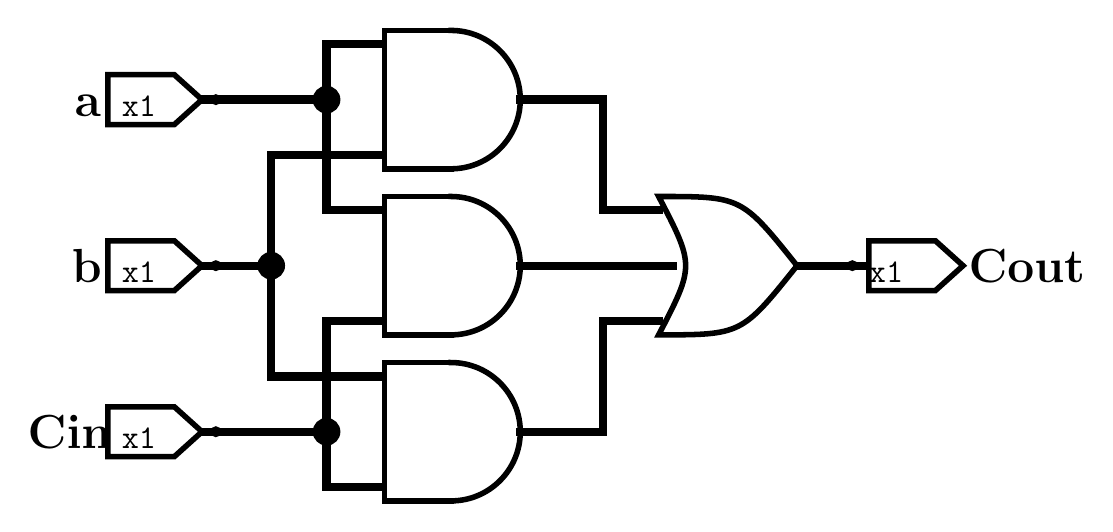
\begin{tikzpicture}[x=1pt,y=-1pt,line cap=rect]
\def\logisimfontA#1{\fontfamily{cmr}{#1}} % Replaced by logisim, original font was "SansSerif"
\def\logisimfontB#1{\fontfamily{cmtt}{#1}} % Replaced by logisim, original font was "Monospaced"
\definecolor{custcol_0_0_0}{RGB}{0, 0, 0}
\definecolor{custcol_ff_ff_ff}{RGB}{255, 255, 255}
\draw [line width=3.0pt, custcol_0_0_0 ]  (283.0,90.0) -- (303.0,90.0) ;
\draw [line width=3.0pt, custcol_0_0_0 ]  (133.0,50.0) -- (93.0,50.0) -- (93.0,90.0) ;
\draw [line width=3.0pt, custcol_0_0_0 ]  (113.0,30.0) -- (113.0,70.0) -- (133.0,70.0) ;
\draw [line width=3.0pt, custcol_0_0_0 ]  (133.0,110.0) -- (113.0,110.0) -- (113.0,150.0) ;
\fill [line width=3.0pt, custcol_0_0_0]  (93.0,90.0) ellipse (5.0 and 5.0 );
\fill [line width=3.0pt, custcol_0_0_0]  (113.0,150.0) ellipse (5.0 and 5.0 );
\fill [line width=3.0pt, custcol_0_0_0]  (113.0,30.0) ellipse (5.0 and 5.0 );
\draw [line width=2.0pt, custcol_0_0_0] (158.0,175.0) arc (90.0:-90.0:25.0 and 25.0 );
\draw [line width=2.0pt, custcol_0_0_0 ]  (158.0,125.0) -- (134.0,125.0) -- (134.0,175.0) -- (158.0,175.0) ;
\draw [line width=2.0pt, custcol_0_0_0] (158.0,115.0) arc (90.0:-90.0:25.0 and 25.0 );
\draw [line width=2.0pt, custcol_0_0_0 ]  (158.0,65.0) -- (134.0,65.0) -- (134.0,115.0) -- (158.0,115.0) ;
\draw [line width=2.0pt, custcol_0_0_0] (158.0,55.0) arc (90.0:-90.0:25.0 and 25.0 );
\draw [line width=2.0pt, custcol_0_0_0 ]  (158.0,5.0) -- (134.0,5.0) -- (134.0,55.0) -- (158.0,55.0) ;
\draw [line width=3.0pt, custcol_0_0_0 ]  (68.0,90.0) -- (73.0,90.0) -- (93.0,90.0) -- (93.0,130.0) -- (133.0,130.0) ;
\draw [line width=2.0pt, custcol_0_0_0 ]  (58.0,99.0) -- (68.0,90.0) -- (58.0,81.0) -- (34.0,81.0) -- (34.0,99.0) -- cycle;
\logisimfontB{\fontsize{12pt}{12pt}\selectfont\node[inner sep=0, outer sep=0, custcol_0_0_0, anchor=base west] at  (39.0,96.0)  {x1};}
\logisimfontA{\fontsize{16pt}{16pt}\fontseries{bx}\selectfont\node[inner sep=0, outer sep=0, custcol_0_0_0, anchor=base west] at  (21.0,96.0)  {b};}
\fill [line width=2.0pt, custcol_0_0_0]  (73.0,90.0) ellipse (2.0 and 2.0 );
\draw [line width=3.0pt, custcol_0_0_0 ]  (68.0,30.0) -- (73.0,30.0) -- (113.0,30.0) -- (113.0,10.0) -- (133.0,10.0) ;
\draw [line width=2.0pt, custcol_0_0_0 ]  (58.0,39.0) -- (68.0,30.0) -- (58.0,21.0) -- (34.0,21.0) -- (34.0,39.0) -- cycle;
\logisimfontB{\fontsize{12pt}{12pt}\selectfont\node[inner sep=0, outer sep=0, custcol_0_0_0, anchor=base west] at  (39.0,36.0)  {x1};}
\logisimfontA{\fontsize{16pt}{16pt}\fontseries{bx}\selectfont\node[inner sep=0, outer sep=0, custcol_0_0_0, anchor=base west] at  (22.0,36.0)  {a};}
\fill [line width=2.0pt, custcol_0_0_0]  (73.0,30.0) ellipse (2.0 and 2.0 );
\draw [line width=3.0pt, custcol_0_0_0 ]  (68.0,150.0) -- (73.0,150.0) -- (113.0,150.0) -- (113.0,170.0) -- (133.0,170.0) ;
\draw [line width=2.0pt, custcol_0_0_0 ]  (58.0,159.0) -- (68.0,150.0) -- (58.0,141.0) -- (34.0,141.0) -- (34.0,159.0) -- cycle;
\logisimfontB{\fontsize{12pt}{12pt}\selectfont\node[inner sep=0, outer sep=0, custcol_0_0_0, anchor=base west] at  (39.0,156.0)  {x1};}
\logisimfontA{\fontsize{16pt}{16pt}\fontseries{bx}\selectfont\node[inner sep=0, outer sep=0, custcol_0_0_0, anchor=base west] at  (5.0,156.0)  {Cin};}
\fill [line width=2.0pt, custcol_0_0_0]  (73.0,150.0) ellipse (2.0 and 2.0 );
\draw [line width=3.0pt, custcol_0_0_0 ]  (183.0,30.0) -- (213.0,30.0) -- (213.0,70.0) -- (233.0,70.0) -- (233.0,70.0) ;
\draw [line width=3.0pt, custcol_0_0_0 ]  (183.0,90.0) -- (233.0,90.0) -- (238.0,90.0) ;
\draw [line width=3.0pt, custcol_0_0_0 ]  (233.0,110.0) -- (233.0,110.0) -- (213.0,110.0) -- (213.0,150.0) -- (183.0,150.0) ;
\draw [line width=2.0pt, custcol_0_0_0 ]  (283.0,90.0) .. controls  (263.0,65.0)  ..  (233.0,65.0) .. controls  (246.0,90.0)  ..  (233.0,115.0) .. controls  (263.0,115.0)  ..  (283.0,90.0) -- cycle ;
\draw [line width=3.0pt, custcol_0_0_0 ]  (307.0,90.0) -- (304.0,90.0) ;
\draw [line width=2.0pt, custcol_0_0_0 ]  (333.0,81.0) -- (343.0,90.0) -- (333.0,99.0) -- (309.0,99.0) -- (309.0,81.0) -- cycle;
\logisimfontB{\fontsize{12pt}{12pt}\selectfont\node[inner sep=0, outer sep=0, custcol_0_0_0, anchor=base west] at  (309.0,96.0)  {x1};}
\logisimfontA{\fontsize{16pt}{16pt}\fontseries{bx}\selectfont\node[inner sep=0, outer sep=0, custcol_0_0_0, anchor=base west] at  (345.0,96.0)  {Cout};}
\fill [line width=2.0pt, custcol_0_0_0]  (303.0,90.0) ellipse (2.0 and 2.0 );
\end{tikzpicture}
}
